\documentclass{beamer}
%[aspectratio=169]   \usepackage[czech]{babel}
\usepackage{apo-lecture-en}
\usepackage{pdfpages}
\usepackage{pdfcomment}
\usepackage{listings}
\usepackage{array,multirow}

\subtitle{Lecture 08. MZ\_APO Educational Kit (Xilinx Zynq MicroZed APO)}
\author{Pavel Píša \phantom{xxxxxxxxx} Petr Štěpán \\ \small\texttt{pisa@fel.cvut.cz}\phantom{xxxx}\small\texttt{stepan@fel.cvut.cz}}
\begin{document}

\maketitle

\section{MZ\_APO -- Xilinx Zynq MicroZed Educational Kit for B35APO}

\begin{frame}
\frametitle{Today's Lecture Objective}

\begin{itemize}
 \item Introduction to the components/construction of the educational kit
 \item Communication and basic work with the kit
 \item Principle and access to the liquid crystal display (LCD)
 \item Color models for rendering
 \item Font output
 \item Use of HW for real applications
\end{itemize}
\end{frame}

\begin{frame}
\frametitle{MZ\_APO Educational Kit -- Assembled}

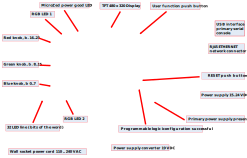
\includegraphics[width=0.98\textwidth]{mz_apo-kit-with-cover-labels-en.pdf}

\end{frame}

\begin{frame}
\frametitle{MZ\_APO Educational Kit -- Mainboard and SBC}

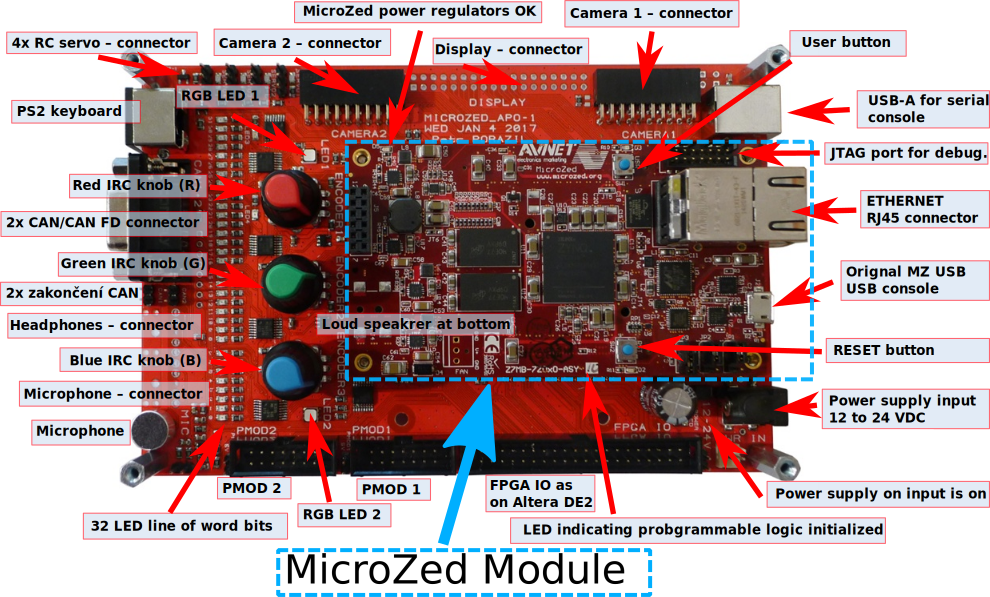
\includegraphics[width=1.0\textwidth]{mz_apo-baseboard-top-labels-en.pdf}

\end{frame}

\begin{frame}
\frametitle{MicroZed SBC (Single Board Computer) -- Top View}

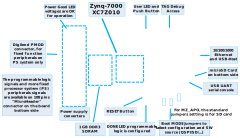
\includegraphics[width=1.0\textwidth]{microzed-board-top-labels-en.pdf}

\end{frame}

\begin{frame}
\frametitle{MicroZed SBC (Single Board Computer) -- Bottom View}

MicroZed Evaluation Kit -- ADSAES-Z7MB-7Z010-G (alternative AES-Z7MB-7Z010-SOM-G/REV-H price 214\,USD)
\par
SoM -- System on Module or SBC (Single Board Computer)
\par
Core SoC Xilinx/AMD XC7Z010, price about 90\,USD (2023)
\par
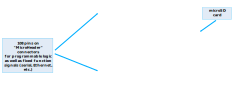
\includegraphics[width=0.90\textwidth]{microzed-board-bottom-labels-en.pdf}
\par
The 108-pin connectors allows use and connect the module with custom design. These connectors are alternative to power the module, allows access the PS peripherals and the programmable logic pins PL (FPGA)

\end{frame}

\begin{frame}
\frametitle{MicroZed Module -- Features Overview}

\begin{itemize}
 \item SoC FPGA – Zynq™-7000 AP SoC (XC7Z010-CLG400-1)
 \begin{itemize}
  \item CPU: Dual ARM® Cortex™-A9 MPCore™ @ 866 MHz
  \item fast internal static memory 256\,kB
  \item 4400 slices - each slice is a small configurable logic circuit.
     It can realize up to 8 flip-flops and 4 logic functions with 6 inputs each.
     The user can freely configure and interconnect them. (28\,K logic blocks, about 430\,K equivalent logic gates)
  \item 240\,KB (60$\times$36\,kbit) RAM a 80$\times$DSP (MAC)

 \end{itemize}
  \item External dynamic memory – 1 GB DDR3
  \item Communication –- 10/100/1000 Ethernet
  \item MicroSD card 4 GB. In APO case, it is used for U-boot to load the Linux kernel over Ethernet.
  \item USB Host 2.0 and USB-UART
  \item Quad-SPI Flash 128\,Mb for initialization at power-on.
  \item Not used in the APO case
\end{itemize}
\end{frame}

\begin{frame}
\frametitle{Zynq™-7000 AP -- SoC FBGA Package}

\begin{columns}
\begin{column}{0.5\textwidth}
  \begin{center}
    FBGA = Fine-Pitch Ball Grid Array
    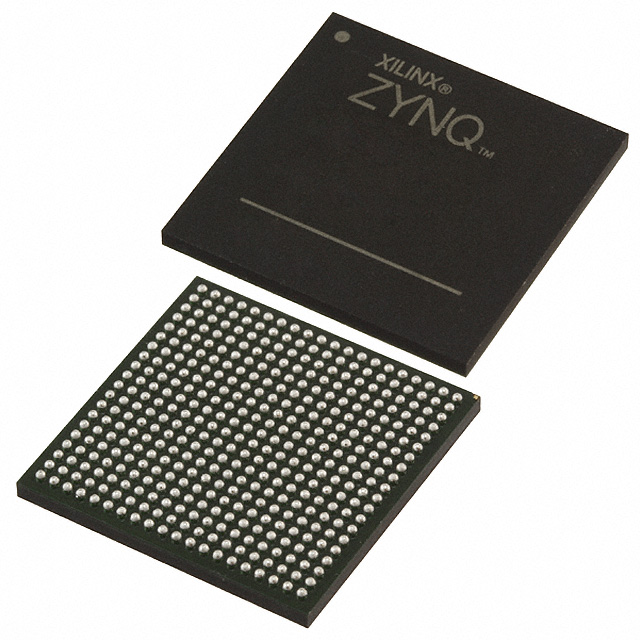
\includegraphics[width=1.0\textwidth]{fig/zynq-fbga-package.jpg}
  \end{center}
  \vfil
\end{column}
\begin{column}{0.5\textwidth}
  \begin{center}
    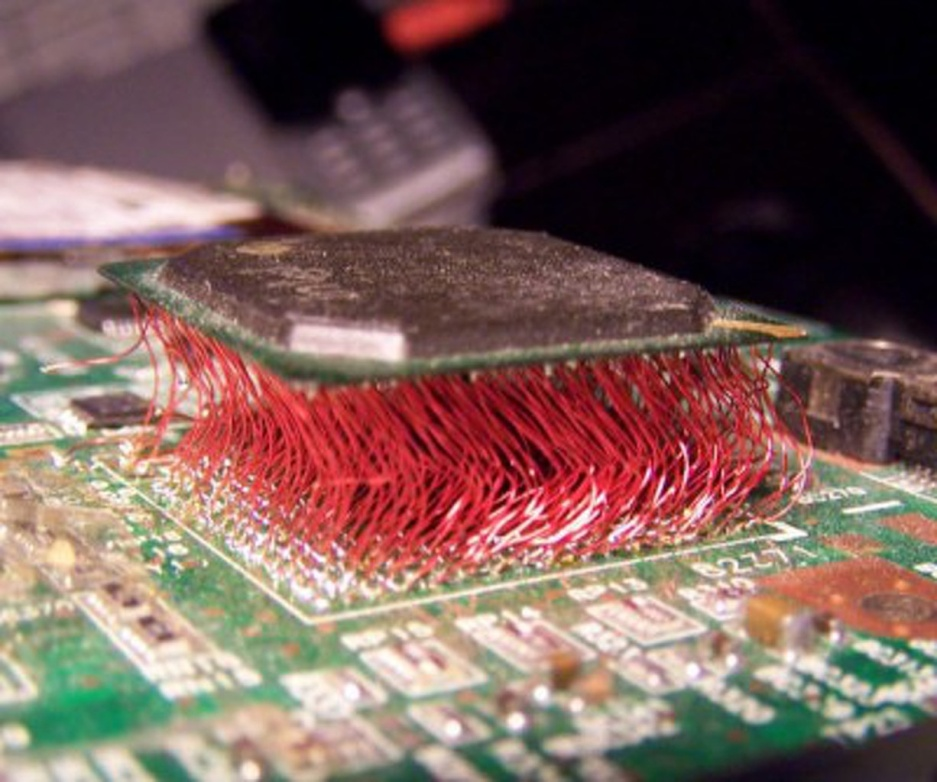
\includegraphics[width=0.55\textwidth]{fig/bga-soldering-clumsy.jpg}
    \newline
    Non-standard soldering as curiosity 
    \newline
    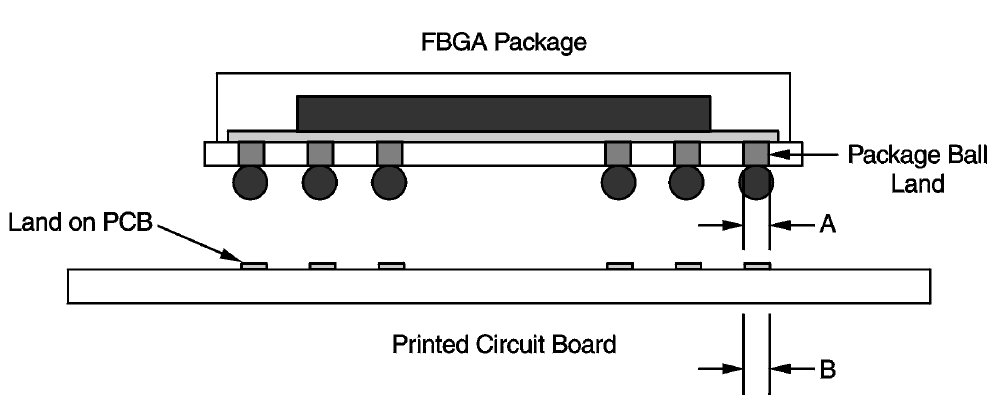
\includegraphics[width=0.8\textwidth]{fig/bga-dimensions-diagram.png}
    \newline
    Standard/correct soldering
    \newline
    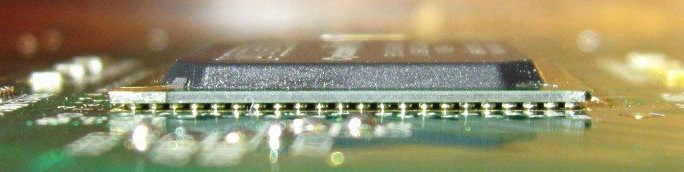
\includegraphics[width=0.8\textwidth]{fig/bga-soldering-proper.jpg}
  \end{center}
\end{column}
\end{columns}

\end{frame}

\begin{frame}
\frametitle{Xilinx Zynq-7000 -- System on Chip (SoC)}
  \begin{center}
    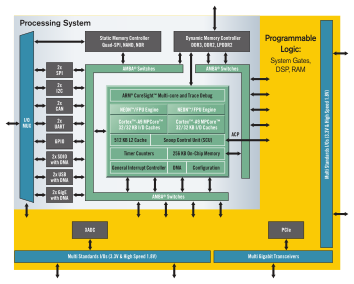
\includegraphics[width=0.73\textwidth]{xylinx-zynq-7000-block-diagram-en.pdf}
  \end{center}
\end{frame}

\begin{frame}
\frametitle{Detailed Processor Cores Block}
\begin{columns}
\begin{column}{0.6\textwidth}
  \begin{center}
    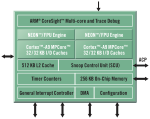
\includegraphics[width=0.95\textwidth]{xylinx-zynq-7000-block-core.pdf}
  \end{center}
  \vfil
\end{column}
\begin{column}{0.4\textwidth}
 {
 %\scriptsize
 \footnotesize
 Already introduced in APO
 \begin{enumerate}
  \item Processor core
  \item Floating point unit (FPU)
  \item Instruction and data level 1 cache
  \item The Level 2 larger common cache
  \item Static memory on chip (RAM)
 \end{enumerate}
 The concepts to learn yet
 \begin{enumerate}
  \item Memory coherence and related Snoop Control Unit
  \item Direct Memory Access for peripherals and accelerators
 \end{enumerate}
 }
\end{column}
\end{columns}
\end{frame}

\begin{frame}
\frametitle{Examples of Consumer Devices with Cortex-A9 Core}

{ \scriptsize
The implementation list \url{https://en.wikipedia.org/wiki/ARM\_Cortex-A9\#Implementations}
}
\vspace{2mm}
\begin{columns}
\begin{column}{0.5\textwidth}
  {\scriptsize
  Asus Transformer Pad, Infinity (TF700T) \tiny \linebreak
  \url{https://en.wikipedia.org/wiki/Asus_Transformer_Pad_Infinity}
  }
  \begin{center}
    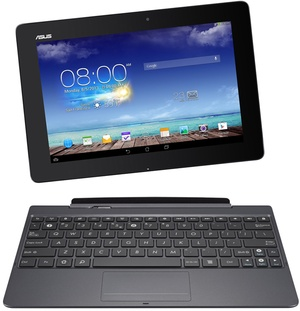
\includegraphics[width=0.7\textwidth]{fig/asus-transformer.jpg}
  \end{center}
\end{column}
\begin{column}{0.5\textwidth}
  {\scriptsize
  Apple A5 (iPhone 4S, iPad 2, iPad mini) \tiny \linebreak
  \url{http://en.wikipedia.org/wiki/Iphone_4s}
  }
  \begin{center}
    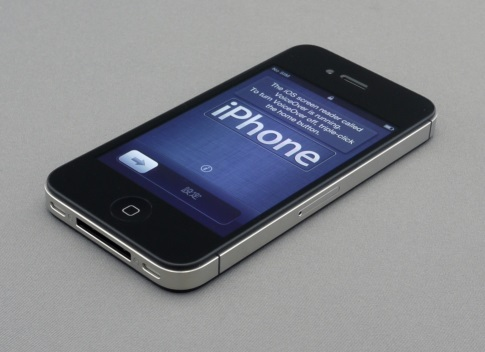
\includegraphics[width=0.5\textwidth]{fig/apple-iphone-with-a5.jpg}
  \end{center}
  {\scriptsize
  NVIDIA Tegra 2 (Motorola Xoom, Droid X2) \tiny \linebreak
  \url{http://en.wikipedia.org/wiki/Motorola_Xoom}
  }
  \begin{center}
    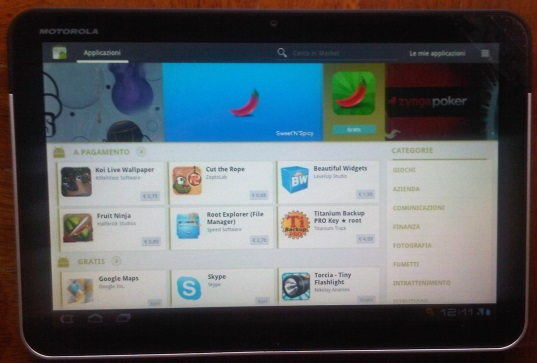
\includegraphics[width=0.4\textwidth]{fig/motorola-xoom.jpg}
  \end{center}
\end{column}
\end{columns}
\end{frame}

\begin{frame}
\frametitle{Cortex-A9 Core Microarchitecture}

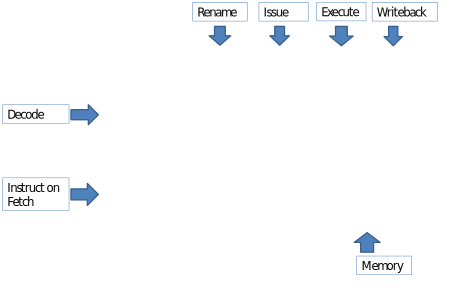
\includegraphics[width=0.95\textwidth]{cortex-a9-core-pipeline-label.pdf}

\end{frame}

\begin{frame}
\frametitle{Zynq Cortex-A9 Parameters}

\begin{itemize}
 \item 32-bit RISC Little Endian, 16 integer registers (GPRs)
 \begin{itemize}
  \item 2.5 DMIPS/MHz $\Rightarrow$ 866 MHz *2.5 DMIPS/MHz = 2165 DMIPS
  {\newline Note: DMIPS -- the Dhrystone synthetic computing benchmark designed to evaluate integer computation performance}
 \end{itemize}
 \item The most of integer operations with 1 cycle latency, integer multiply 4 or 5 cycles.
 \item Floating point operations pass through ALU in 4 cycles for addition and subtraction (FADD, FSUB), 5 cycles required for multiplication FMUL, 15 cycles for division FDIV (3x more than multiplication!), 17 cycles a second root square FSQRT.
 \item Branch prediction
 \begin{itemize}
  \item 4\,K 2-bit predictors in the branch history table
 \end{itemize}
 \item MMU for virtual memory with 2 two page table levels
\end{itemize}

\end{frame}

\begin{frame}
\frametitle{Cache Memory Level 1 and Level 2}
\begin{itemize}
 \item two independent L1 caches for each core, I-cache for instructions and D-cache for data. Common L1 cache parameters:
 \begin{itemize}
  \item capacity/size: 32\,kB
  \item 4-way set associative
  \item block/row size: 32 bytes
  \item pseudo-random or pseudo round-robin replacement policy
  \item D-Cache supports write-back/write-allocate policy variants.
 \end{itemize}
 \item L2 Cache is shared by both Cortex-A9 Cores. Parameters:
 \begin{itemize}
   \item capacity/size> 512\,kB
   \item 8-way set associative
   \item block/row size: 32 bytes
   \item pseudo-random replacement policy
   \item supports write-back and write-through (with and without allocation)
 \end{itemize}
\end{itemize}

\end{frame}

\begin{frame}
\frametitle{Two Levels Paging, Reminder from Lecture 4 for x86}

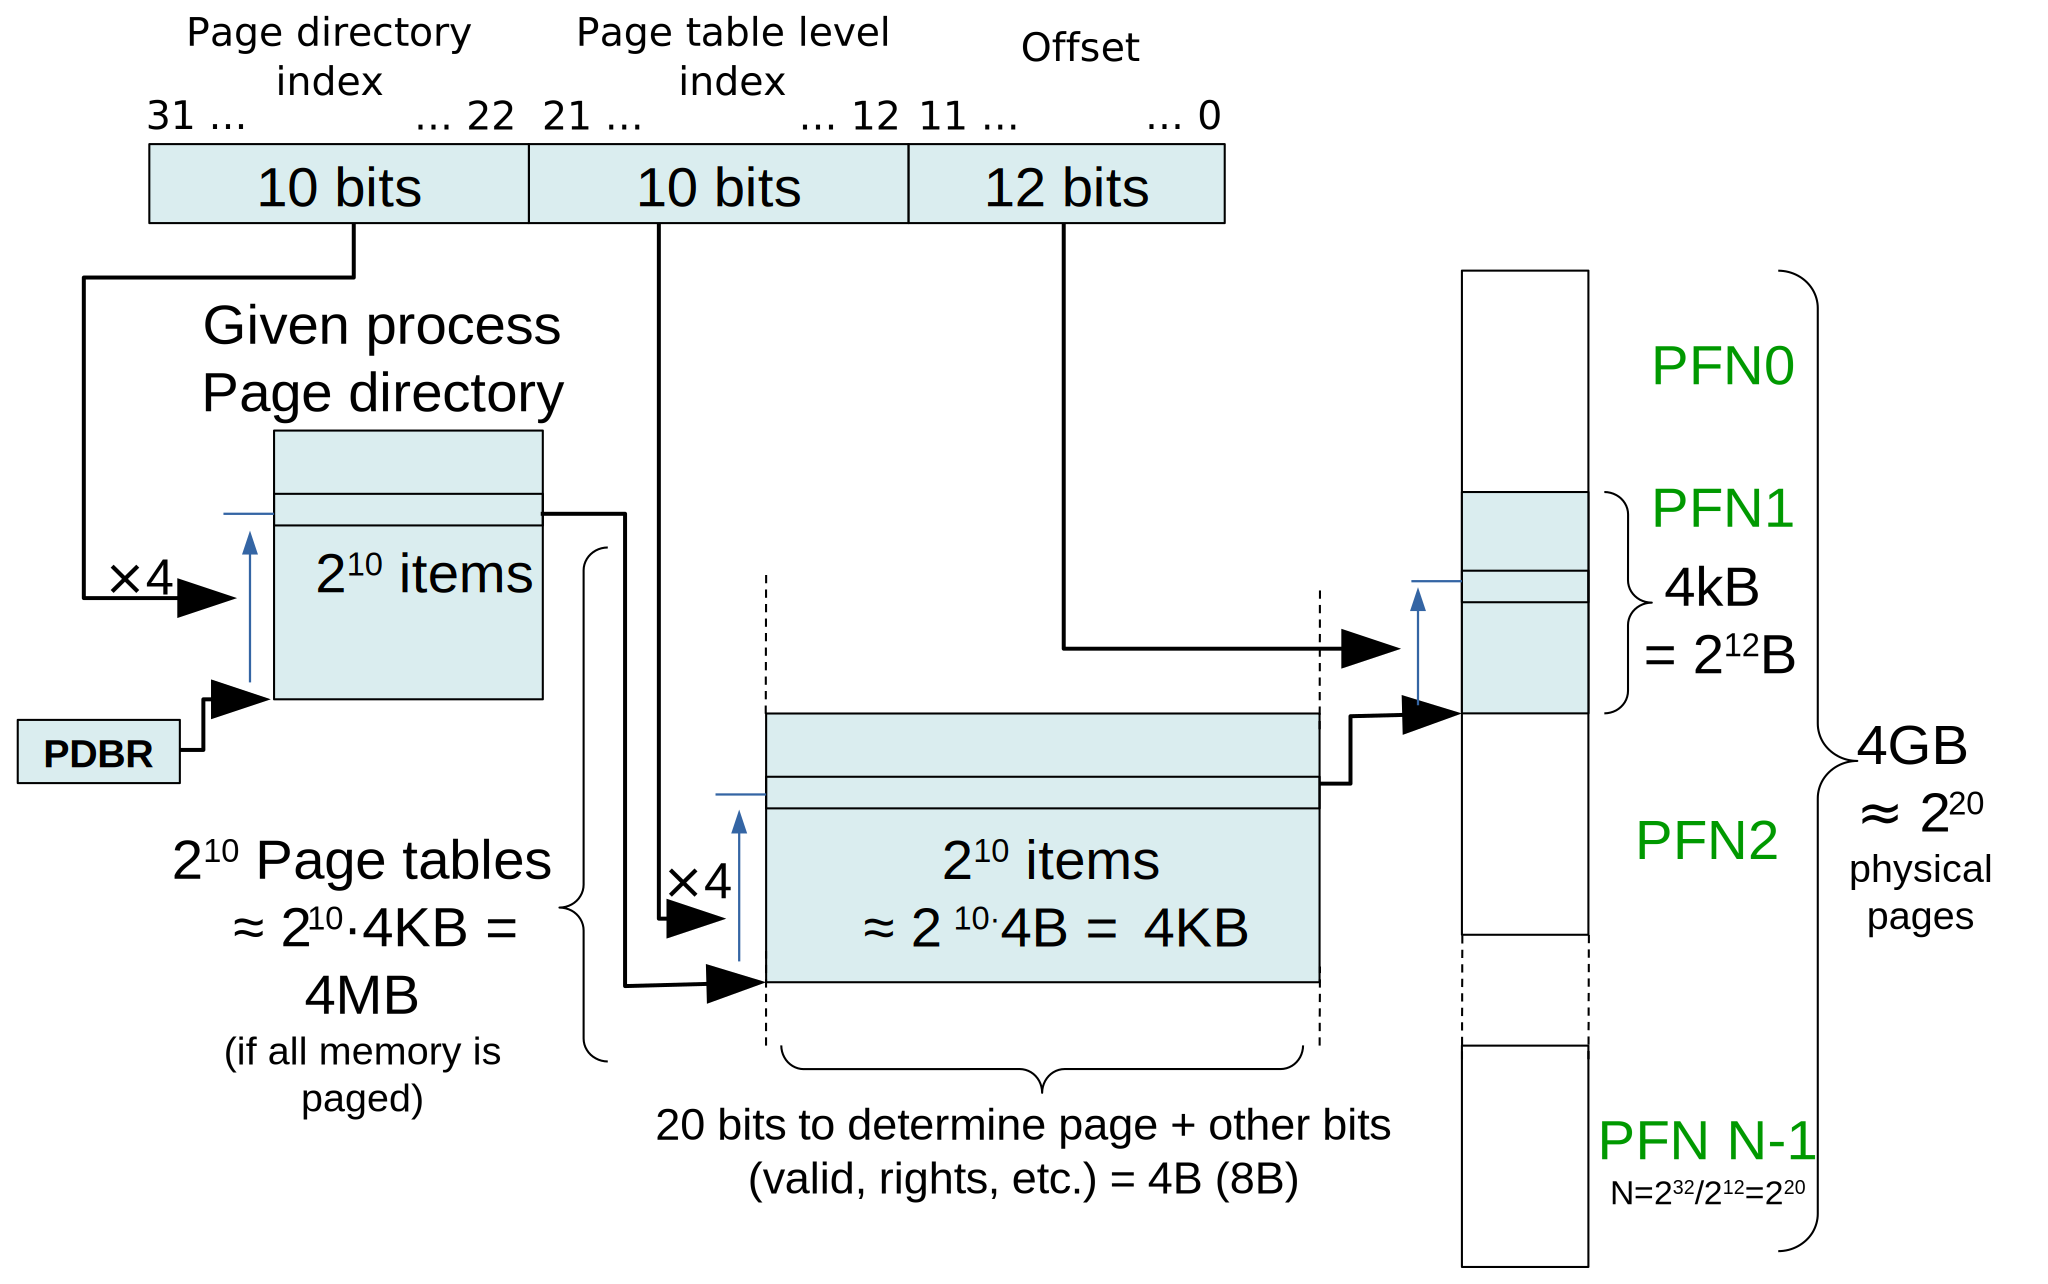
\includegraphics[width=1.0\textwidth]{paging-2-levels-en.pdf}

\end{frame}

\begin{frame}
\frametitle{Two Level Paging on ARM Cortex-A9, Asymmetric Indexes}

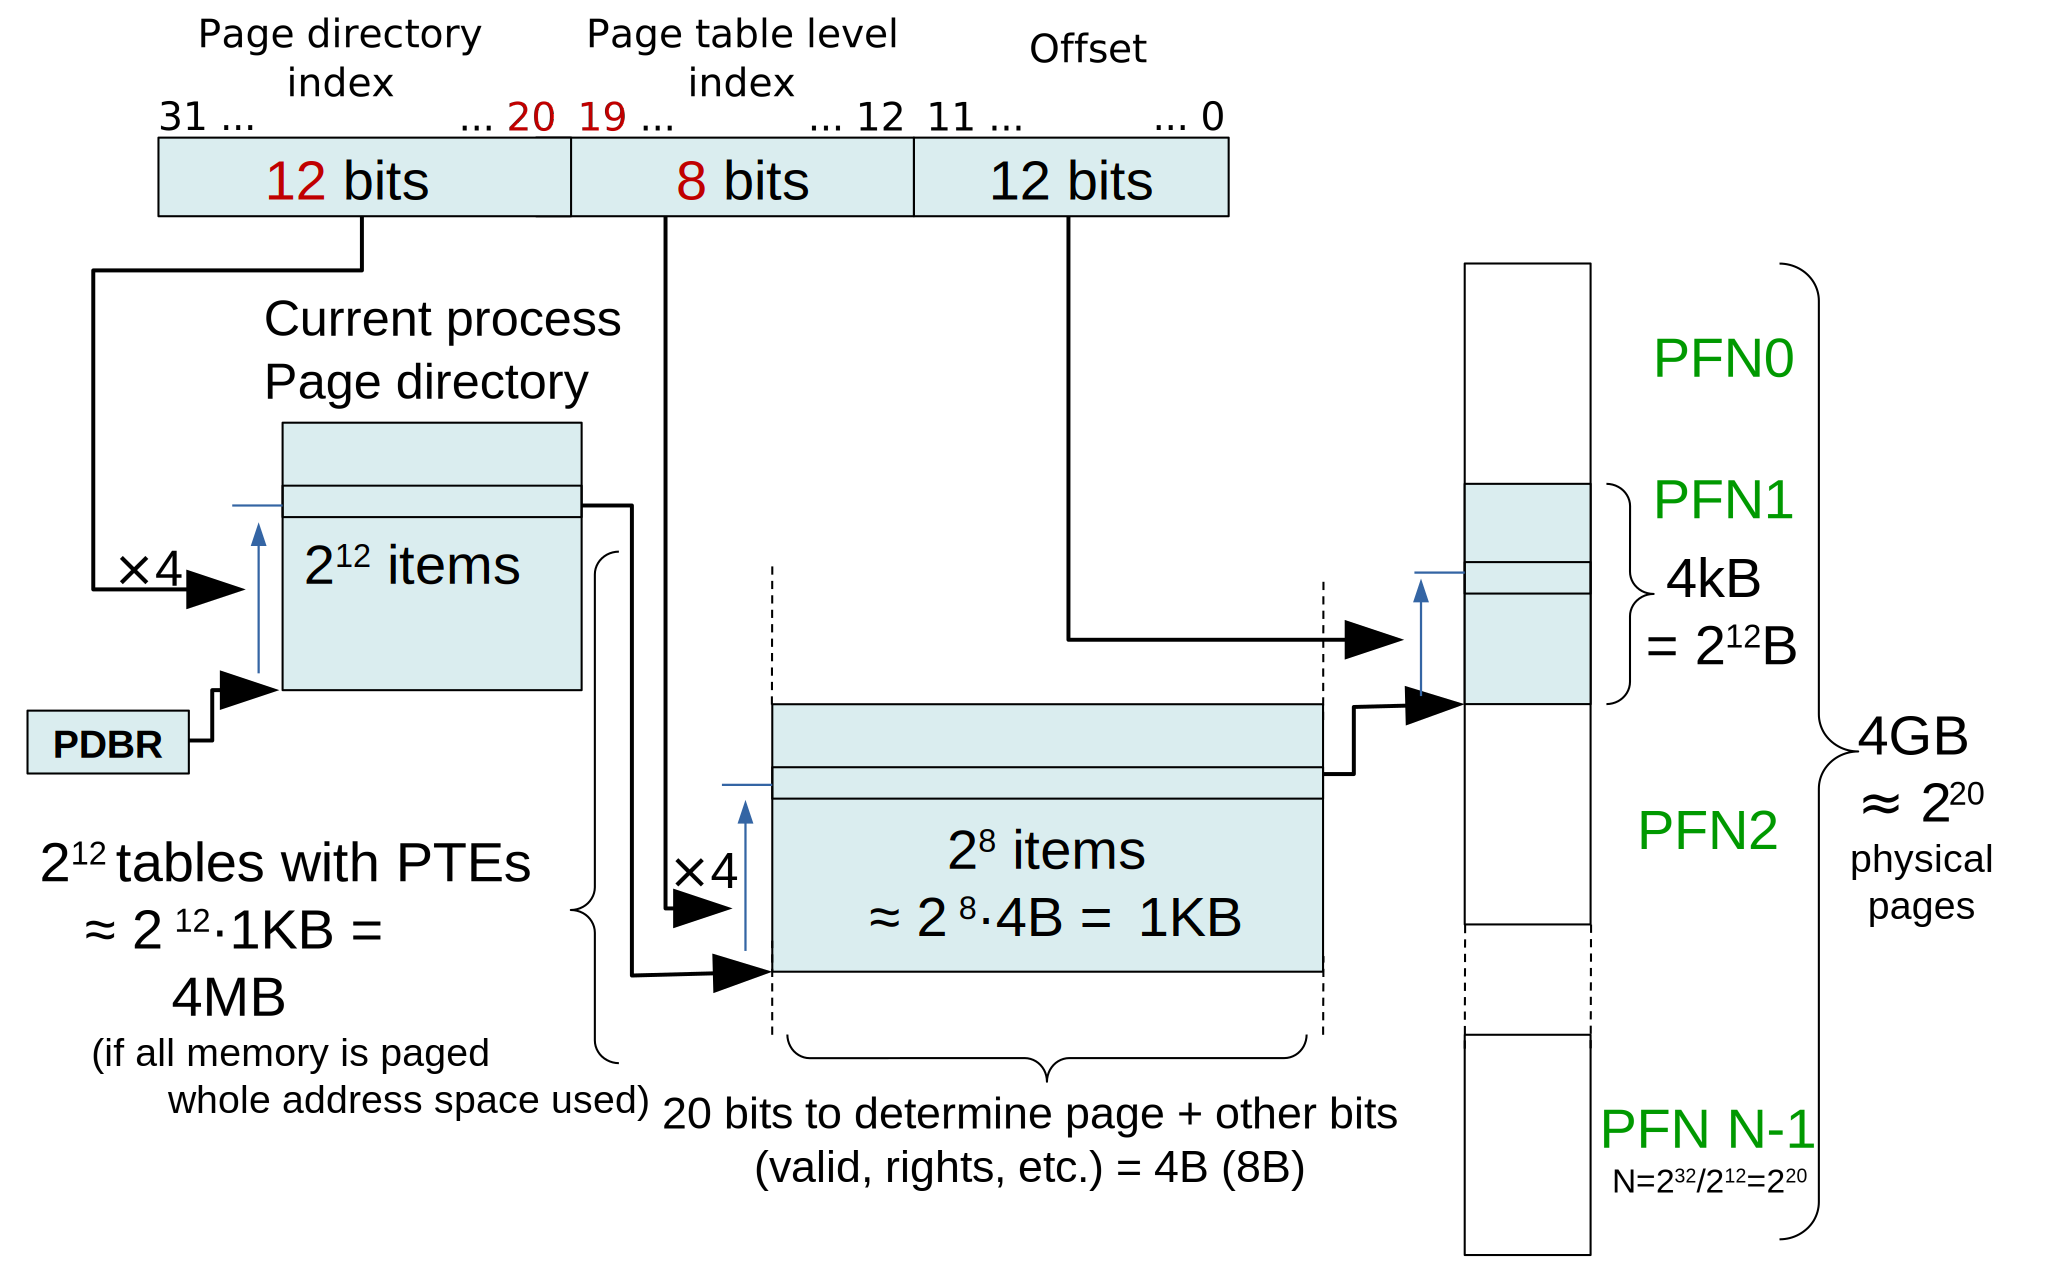
\includegraphics[width=1.0\textwidth]{paging-2-levels-cortex-a9-en.pdf}

\end{frame}

\section{MZ\_APO -- Memory Mapped Peripherals in CPU Address Space}

\begin{frame}
\frametitle{Memory Mapped Peripherals -- Reminder}

\begin{itemize}
\item There are no input/output specific instructions on ARM
\item Memory load and store instructions are used for peripheral accesses
\item Address Decoder -- controls where are data routed
\end{itemize}
\begin{center}
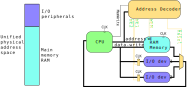
\includegraphics[width=0.88\textwidth]{address_decoder-en.pdf}
\end{center}
\end{frame}

\begin{frame}
\frametitle{AMBA AXI Interconnect Bus -- Channels Principle}

\begin{center}
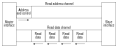
\includegraphics[width=0.55\textwidth]{amba-axi-read-concept-en}
\end{center}

\begin{center}
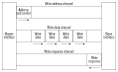
\includegraphics[width=0.55\textwidth]{amba-axi-write-concept-en}
\end{center}

\footnotesize{AMBA -- Advanced Microcontroller Bus Architecture \\ AXI -- Advanced eXtensible Interface}

\end{frame}

\begin{frame}
\frametitle{AMBA AXI Bus -- Read Transaction}

\begin{center}
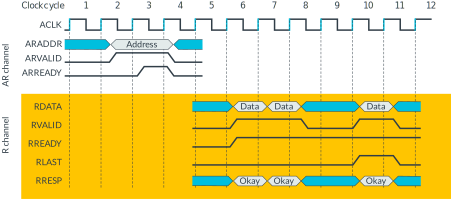
\includegraphics[width=1.0\textwidth]{amba-axi-read.pdf}
\end{center}

\begin{itemize}
\item Independent channels for address and data
\item The word transfer is realized when both, xVALID and xREADY, are asserted
\end{itemize}

\end{frame}

\begin{frame}
\frametitle{AMBA AXI Bus -- Write Transaction}

\begin{center}
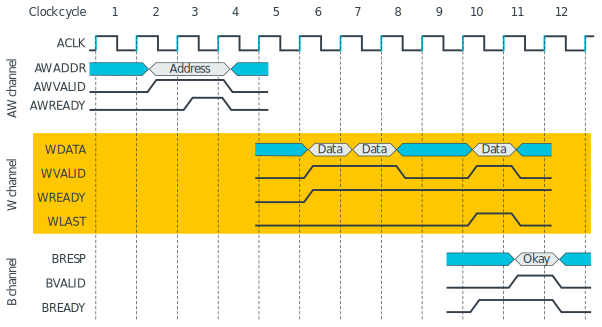
\includegraphics[width=1.0\textwidth]{amba-axi-write.pdf}
\end{center}

\end{frame}

\begin{frame}
\frametitle{MZ\_APO Logic Design in Vivado System}
  \begin{center}
    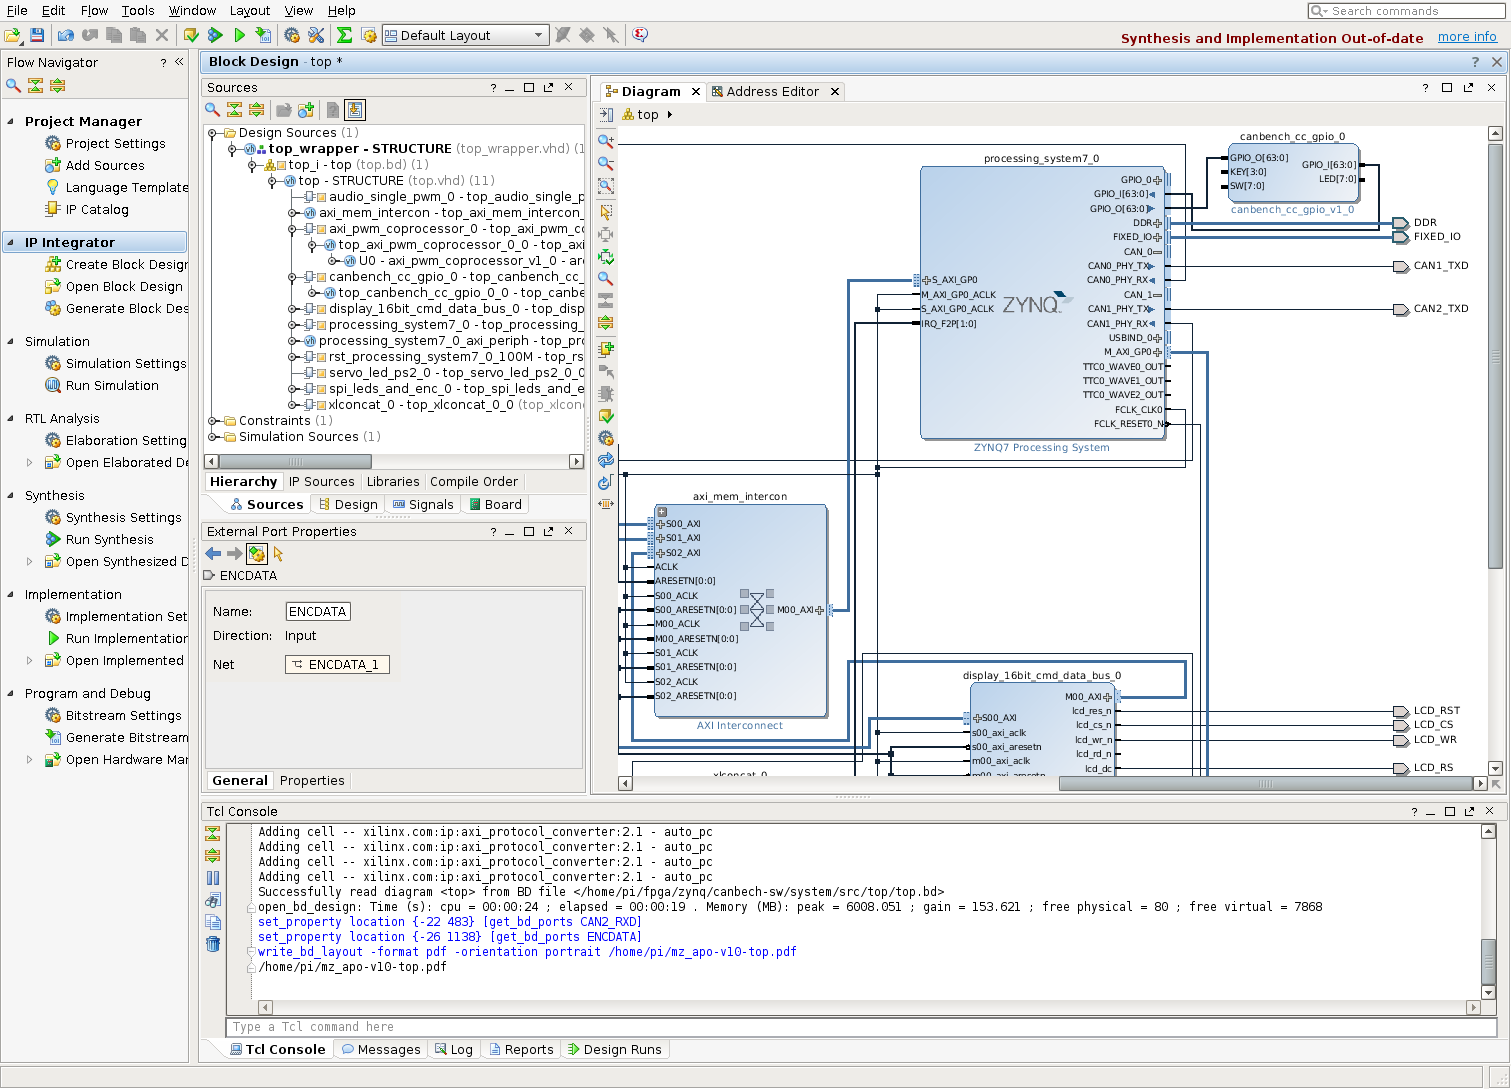
\includegraphics[width=0.8\textwidth]{fig/mz_apo-vivado-screenshot.png}
  \end{center}
\end{frame}

\begin{frame}
\frametitle{MZ\_APO Logic Design -- Interconnection of the Blocks and IP Cores by Signals and AXI Buses}

\includegraphics[width=1.0\textwidth]{mz_apo-vivado-design.pdf}

\end{frame}

\begin{frame}
\frametitle{MZ\_APO -- Physical Addresses of Educational Peripherals}

\begin{tabular}{|l|l|l|l|} \hline
Base address & Range & Mapped Function \\\hline
0x0000 0000 & 1 GB &  DRAM \\\hline
0x4000 0000 & 1 GB & AXI port 0 to connect programmable part \\\hline
\textbf{0x43c0 0000} & 16 bytes & \textbf{APO -- LCD display} \\\hline
0x43c2 0000 & 32 bytes & DC motor connected to PMOD1 \\\hline
0x43c3 0000 & 32 bytes & DC motor connected to PMOD2 \\\hline
\textbf{0x43c4 0000} & 48 bytes & \textbf{APO -- knobs and LEDs peripheral} \\\hline
0x43c5 0000 & 32 bytes & 4$\times$ RC servos and PS2 keyboard \\\hline
0x43c6 0000 & 32 bytes & simple audio \\\hline
0x8000 0000 & 1 GB & AXI port 1 to connect programmable part \\\hline
0xE000 0000 &      & Reserved for system peripherals\\\hline
0xFFFC 0000 &      & 256 kB internal RAM \\\hline

\end{tabular} 

\end{frame}


\begin{frame}
\frametitle{The Physical Address Range Mapping to The Process Virtual Address Space}

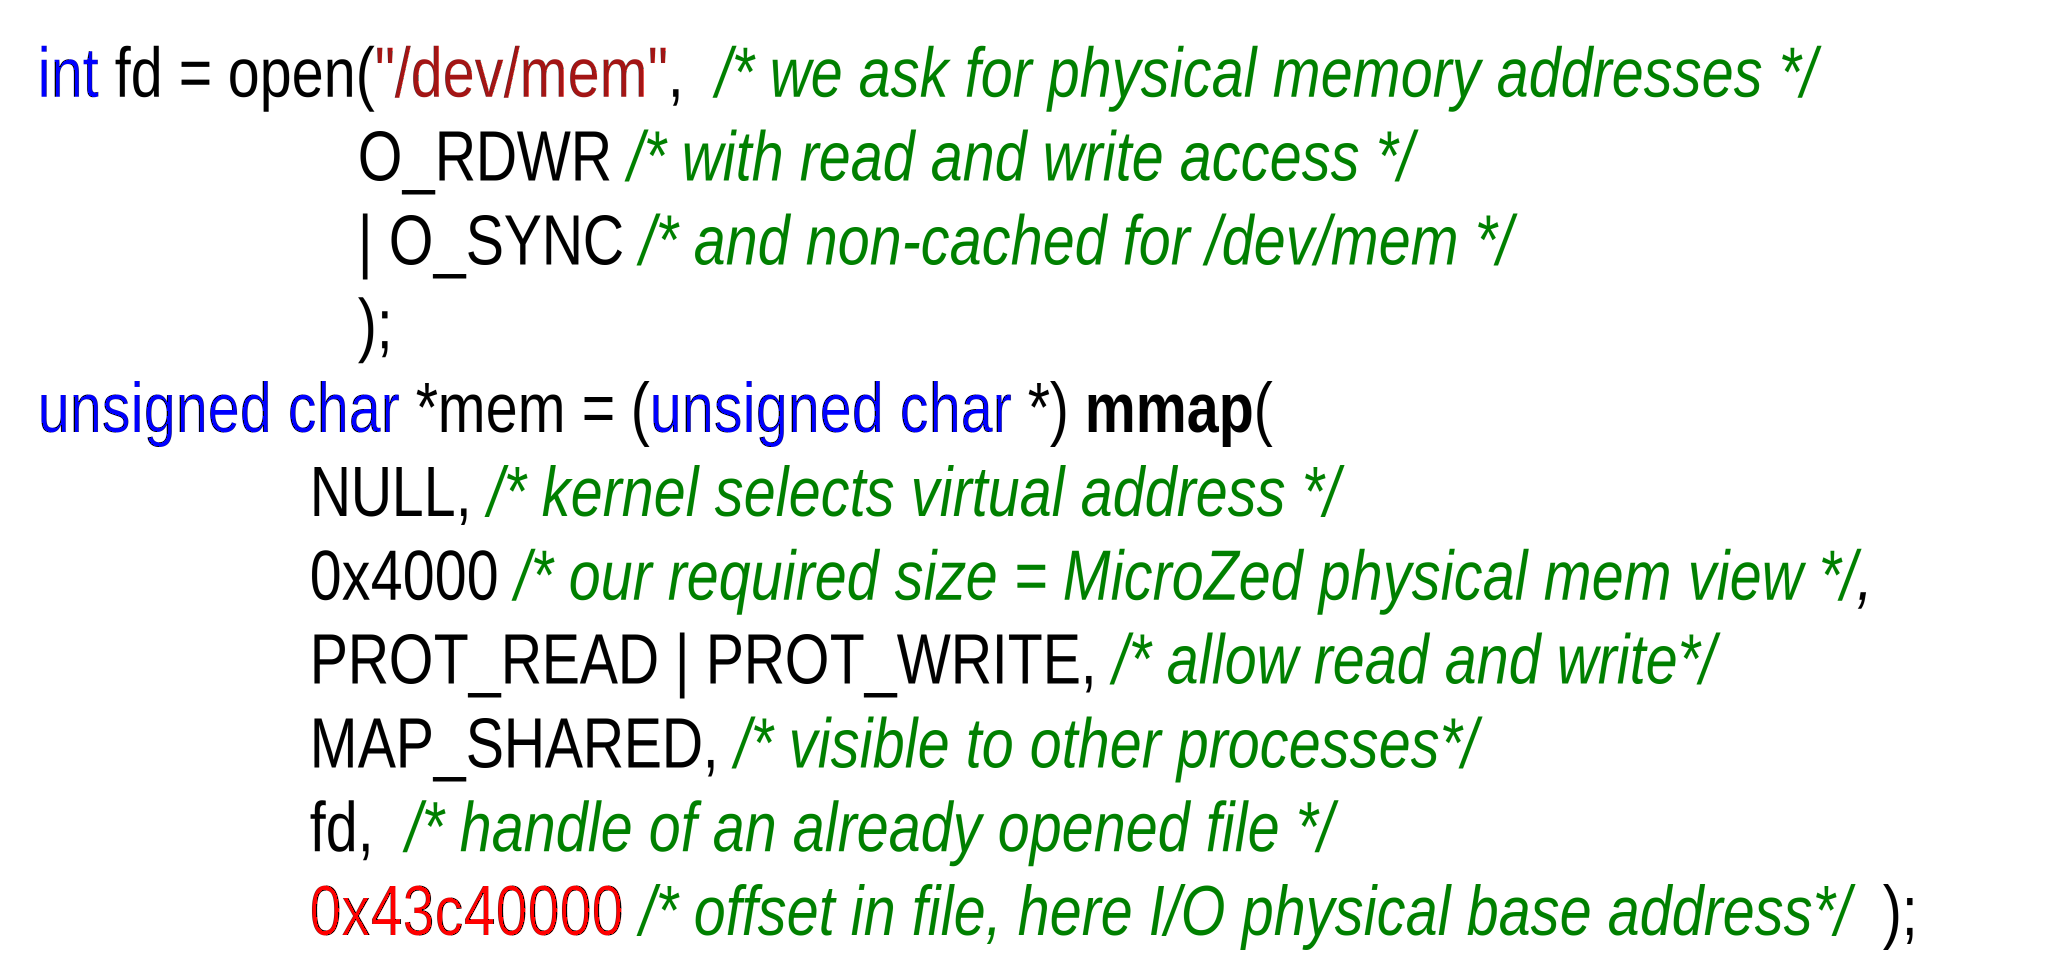
\includegraphics[width=1.0\textwidth]{mmap-phys-memory-range-en.pdf}

\end{frame}

\begin{frame}
\frametitle{MZ\_APO -- LED Line, RGB LEDs and Rotary Knobs}

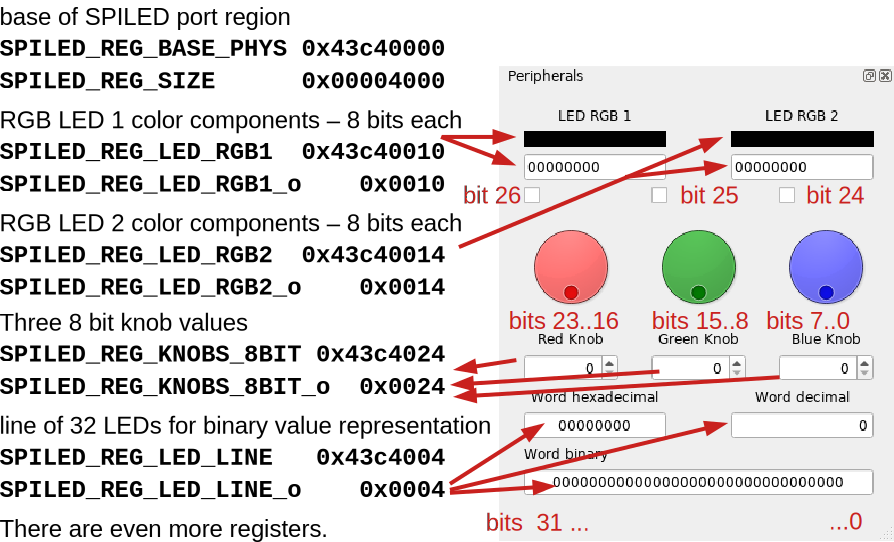
\includegraphics[width=1.0\textwidth]{mz_apo-spiled-and-knobs-en.pdf}

\end{frame}

\begin{frame}
\frametitle{MZ\_APO -- Write Pixels to LCD Display}

Finite state machine (FSM) converts AXI writes to LCD parallel bus and LCD controller chip with local memory. The controller generate signals to periodically refresh LCD TFT display matrix.
When the next AXI write is requested before ongoing transfer is finished then the new one is delayed by AXI READY signal negation until next command/data can be accepted

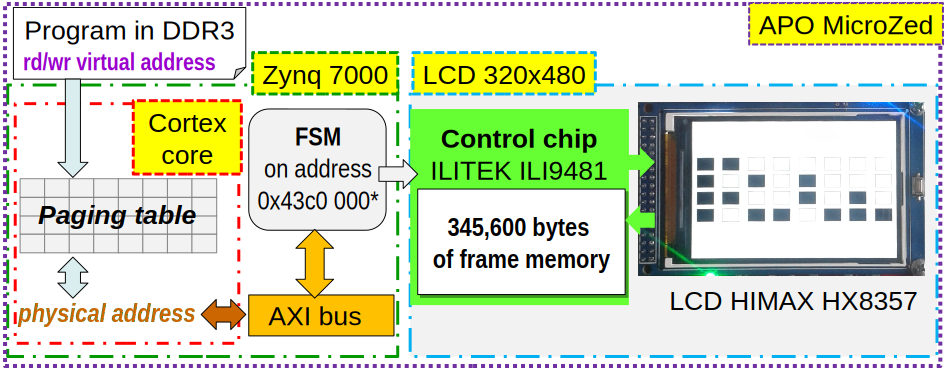
\includegraphics[width=0.9\textwidth]{mz_apo-lcd-access-en.pdf}

\end{frame}

\begin{frame}
\frametitle{MZ\_APO -- Write to LCD Display}

\begin{tabular}{|l|l|l|l|} \hline
Offset & \footnotesize{Data type} & Description \\\hline
+0x0 & \footnotesize{uint16\_t} & \footnotesize{0x1 - reset display controller, bit0 == 0 - no operation} \\\hline
+0x8 & \footnotesize{uint16\_t} & \footnotesize{control command, 0x2c fill pixels from beginning} \\\hline
+0xC & \footnotesize{uint16\_t} & \footnotesize{write 16 bit pixel color (RGB565) or other data} \\\hline
+0xC & \footnotesize{uint32\_t} & \footnotesize{write 2 two pixels: the first bits 15..0, bits 31..16 following one} \\\hline
\end{tabular}

\vspace{5mm}

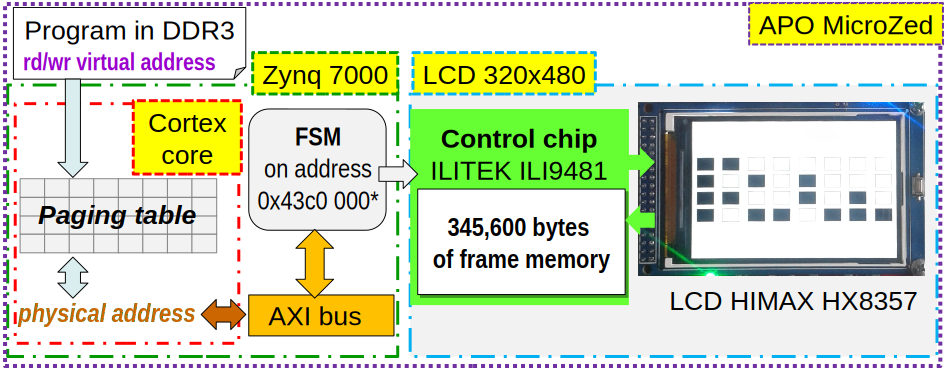
\includegraphics[width=0.9\textwidth]{mz_apo-lcd-access-en.pdf}

\end{frame}

\section{Text Output on Displays}


\begin{frame}
\frametitle{The Font Size and Spacing}

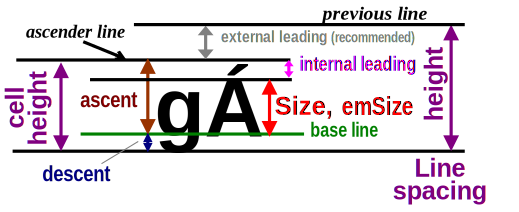
\includegraphics[width=0.98\textwidth]{font-sizes-en.pdf}

If the font does not have diacritics, then it has a zero internal leading and its ascent matches emSize

\end{frame}


\begin{frame}
\frametitle{Bitmap Fonts}

Bitmaps font are faster and easier to use and therefore suitable for low cost computer systems. 

\begin{columns}
\begin{column}{0.35\textwidth}
  \begin{center}
    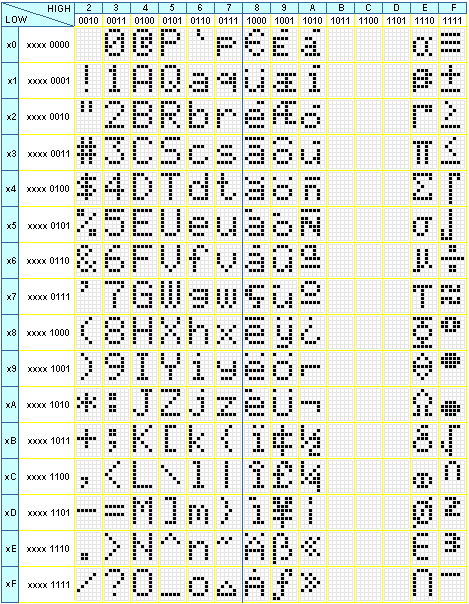
\includegraphics[width=1.0\textwidth]{fig/bitmap-font-encoding-table.png}
  \end{center}
  \vfil
\end{column}
\begin{column}{0.55\textwidth}
  \begin{center}
    \tiny{\url{http://mobilefonts.sourceforge.net/}}

    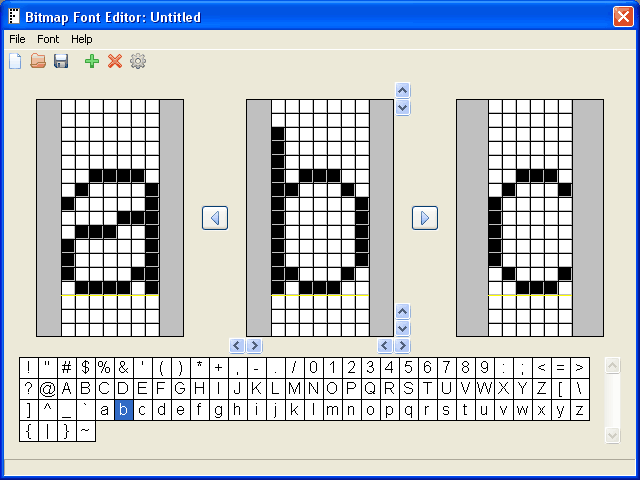
\includegraphics[width=1.0\textwidth]{fig/bitmap-font-abc-example.png}
  \end{center}
  \vfil
\end{column}
\end{columns}

Note: In 1968, the first bitmap font was created by German inventor Rudolf Hell for his Digiset typesetting machine.

\end{frame}


\begin{frame}
\frametitle{The Scalable Font Wars}

\begin{itemize}
\item
  Apple and Microsoft developed (1980) the \textbf{TrueType} methodology
  that is a system of scalable outline fonts, and can draw characters at
  low resolution.
\item
  Adobe \textbf{PostScript} (1984) is another method of describing an
  image in terms of \emph{\textbf{mathematical constructs}} (Bézier
  curves), so it is used not only to describe the individual characters
  of a font but also to describe entire illustrations and whole pages of
  text.
\item
  \textbf{Open Type} (1996) digital font format was developed jointly by
  Apple and Microsoft to put an end to the PostScript/TrueType war.
  ~Like TrueType, a single file contains all the outline and bitmap data
  for an OpenType font, but it also contains either PostScript data or
  additional TrueType data within the font, which in the PostScript
  case, makes the font truly scalable and exacting.
\end{itemize}

Source: wordpress.com

\end{frame}


\begin{frame}
\frametitle{Font Rendering from Geometry to Raster}

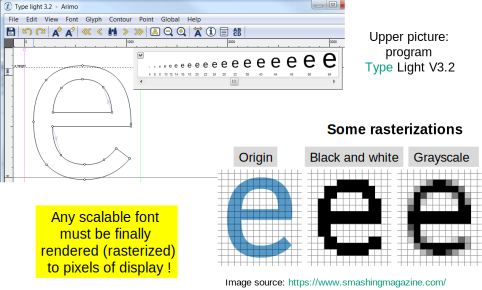
\includegraphics[width=.98\linewidth,height=0.95\textheight,clip=true,keepaspectratio]{font-render-example.pdf}

\end{frame}


\begin{frame}
\frametitle{Black and White Rastered Fonts}

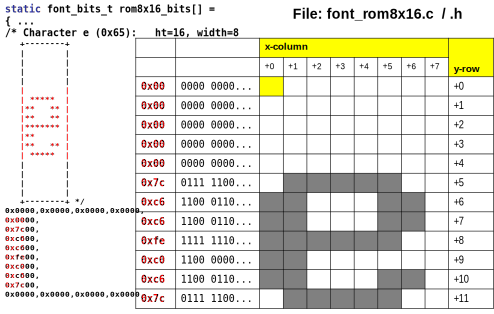
\includegraphics[width=.98\linewidth,height=0.98\textheight,clip=true,keepaspectratio]{font-render-rom8x16.pdf}

\end{frame}

\begin{frame}
\frametitle{Raster Fonts for Use in Semestral Work}

{\small
See: \url{https://gitlab.fel.cvut.cz/b35apo/mzapo_template/}

}

{\small
The raster fonts bitmaps and widths are provided for semestral work. The
fonts are defined in the format used by Microwindows/Nano-X library by
Greg Haerr

\url{https://github.com/ghaerr/microwindows}

}

{\small
The simplified structure to describe font is provided in file

}

{\tiny
\url{https://gitlab.fel.cvut.cz/b35apo/mzapo_template/-/blob/master/font_types.h}

}

{\small
The example of the device where PiKRON has used the Microwindows, RTEMS
and this font definitions from which provided example is simplified

}

\begin{columns}
\begin{column}{0.45\textwidth}
  \begin{center}
     TECHNIC-I

    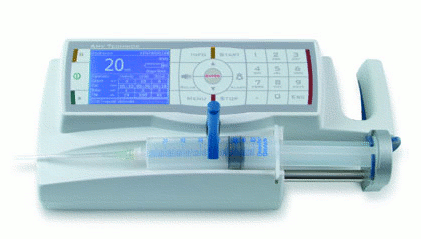
\includegraphics[width=1.0\textwidth]{fig/technic1-photo.png}
  \end{center}
  \vfil
\end{column}
\begin{column}{0.40\textwidth}
  \begin{center}
    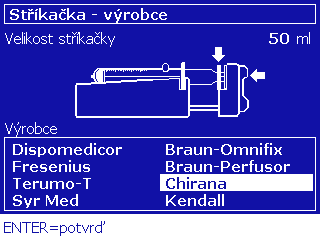
\includegraphics[width=1.0\textwidth]{fig/technic1-screen-syringe.png}
  \end{center}
  \vfil
\end{column}
\end{columns}

{\small \url{https://www.rtems.org/applications/hardware/amv_technic_i/}}

\end{frame}


\begin{frame}
\frametitle{Structure font\_descriptor\_t}

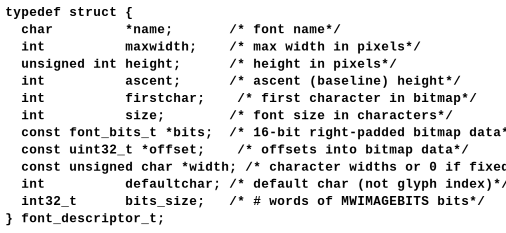
\includegraphics[width=.98\linewidth,height=0.85\textheight,clip=true,keepaspectratio]{font-mw-descriptor.pdf}

\vfill

\href{https://gitlab.fel.cvut.cz/b35apo/mzapo_template/}{https://gitlab.fel.cvut.cz/b35apo/mzapo\_template/}

\end{frame}


\section{MZ\_APO Educational Kit Sources and Use in Projects}


\begin{frame}
\frametitle{MZ\_APO Education Kit Sources}

\begin{itemize}
\item The MZ\_APO education kit has been designed by
\begin{itemize}
\item Petr Porazil
  (\href{mailto:porazil@pikron.com}{\nolinkurl{porazil@pikron.com}}) and
\item Pavel Píša
  (\href{mailto:pisa@cmp.felk.cvut.cz}{\nolinkurl{pisa@fel.cvut.cz}},
  \href{mailto:ppisa@pikron.com}{\nolinkurl{ppisa@pikron.com}}) \\
\end{itemize}
  on request of \href{https://dce.fel.cvut.cz/}{Department of Control
  Engineering (K13135)} former IIG head
\item The complete design files for base board and mechanics are available
  from the repository \\
  \href{https://gitlab.com/pikron/projects/mz_apo/microzed_apo}{https://gitlab.com/pikron/projects/mz\_apo/microzed\_apo}
\item Petr Porazil's electronic design automation PEDA has been used for
  electronics design \\
  \url{https://sourceforge.net/projects/peda/}
\item FPGA design by Pavel Pisa and Martin Jeřábek is available from
  \href{http://canbus.pages.fel.cvut.cz/}{CTU FEE CAN bus} project repositories \\
  \small{\url{https://gitlab.fel.cvut.cz/canbus/zynq/zynq-can-sja1000-top}}
\item the actual design is available on \\
  \href{https://gitlab.fel.cvut.cz/canbus/zynq/zynq-can-sja1000-top/-/commits/microzed_apo_psr}{microzed\_apo\_psr}  branch
\end{itemize}

\end{frame}


\begin{frame}
\frametitle{MZ\_APO Education Kit Sources -- Software}

\begin{itemize}
\item The Linux kernel 4.19 with fully preemptive patches is actually
  running on the boards. The branch
  \href{https://github.com/ppisa/linux-kernel/commits/linux-4.19.y-pi}{linux-4.19.y-pi}
  with integrated patches is available from repository \\
  \url{https://github.com/ppisa/linux-kernel}
\item
  The build is available \\
  \url{https://github.com/ppisa/zynq-rt-utils-and-builds}
\item
  More MZ\_APO documentation prepared for B35 Computer Architectures is
  available \\
  \url{https://cw.fel.cvut.cz/wiki/courses/b35apo/documentation/mz_apo/start}
\item
  MicroZed SBC documentation in Avnet MicroZed HW Users Guide
\end{itemize}

\end{frame}


\begin{frame}
\frametitle{MZ\_APO Education Kit Support Files and Projects}

\begin{itemize}
\item The Simulink and other projects for the boards - more \\
      \url{https://github.com/aa4cc/zynq-rt-control}
\begin{itemize}
\item PMSM control project using Matlab/Simulink \\
      simulink/mz\_apo-3pmdrv/zynq\_pmsm\_motor\_control.slx
\item The hardware design Petr Porazil
  (\href{mailto:porazil@pikron.com}{\nolinkurl{porazil@pikron.com}})
\item Design files hw/prj/fel/motor-driver-1.tdb from the repository \\
  \url{https://gitlab.com/pikron/projects/mz_apo/microzed_apo}
\item FPGA design Pavel Pisa, Marek Peca, Martin Prudek \\
  \href{https://dspace.cvut.cz/bitstream/handle/10467/62036/F3-BP-2015-Prudek-Martin-Bp_2015_prudek_martin.pdf}{Brushless motor control with Raspberry Pi board and Linux}
\end{itemize}
\item The more description of Matlab/Simulink code generation for Linux \\
  \url{http://lintarget.sourceforge.net/}
\item Alternative (Matlab/Simulink independent) robotic motion control project \\
  \url{https://gitlab.com/pikron/projects/pxmc-linux} \\
  which is based on PXMC library \url{http://pxmc.org/}
\end{itemize}

\end{frame}


\begin{frame}
\frametitle{Presentations of Projects Done on MZ\_APO System}

\begin{itemize}
\item LinuxDays 2015, Linux, RPi and other HW for DC and Brushless/PMSM Motor Control,
\href{https://www.linuxdays.cz/2015/video/Pavel_Pisa-Rizeni_stejnosmernych_motoru.pdf}{Slides},
\href{https://youtu.be/uMfY-sKf0HA}{Video} in Czech

\item InstallFest 2017, GNU/Linux and FPGA in Real-time Control Applications,
\href{https://installfest.cz/if17/slides/so_t2_pisa_realtime.pdf}{Slides},
\href{https://youtu.be/sNtlEysC0yA}{Video} in Czech

\item  LinuxDays 2017, GNU/Linux, CAN and CANopen in Real-time Control
Applications,
\href{https://www.linuxdays.cz/2017/video/Pavel_Pisa-CAN_canopen.pdf}{Slides},
\href{https://youtu.be/hYC-XznyOlQ}{Video} in Czech

\item InstallFest 2020, Embedded Linux, FPGA and Motion Control Hands-On
\url{https://pretalx.installfest.cz/installfest-2020/talk/HSNJCM/}

\item Dion Beqiri thesis
\href{https://dspace.cvut.cz/bitstream/handle/10467/101599/F3-BP-2022-Beqiri-Dion-bachelor_thesis_DionBeqiri.pdf}{Open Rapid Control Prototyping, Education and Design Tools} pysimCoder
(\url{https://github.com/robertobucher/pysimCoder}) includes
\href{https://github.com/robertobucher/pysimCoder-examples/tree/main/Linux-mzapo/DCmotor}{examples}
and blocks to control DC on MZ\_APO

\end{itemize}

\end{frame}


\begin{frame}
\frametitle{Articles About GNU/Linux Use for RT Control on Root.cz in Czech}

\href{https://www.root.cz/}{https://www.root.cz/}

\begin{itemize}
\item
  GNU/Linux pro řízení a rychlost jeho odezvy -
  \href{https://www.root.cz/clanky/gnu-linux-pro-rizeni-a-rychlost-jeho-odezvy/}{link}
\item
  Linux pro řízení: minimalistické řešení řízení stejnosměrného mo­toru
  -
  \href{https://www.root.cz/clanky/linux-pro-rizeni-minimalisticke-reseni-rizeni-stejnosmerneho-motoru/}{link}
\end{itemize}

\end{frame}

\end{document}

